\chapter{软件可信性分配}
\label{ch4}

\begin{kaishu}
对轨道交通联锁软件全生命周期进行可信评估之后,根据评估结果,发现问题,对于每个阶段做的不完善的地方提供改进意见。属性,子属性,度量元是要改进的指标对象,度量元是不可分解的最小单元,因此,通过改进度量元来实现改进子属性和属性的目标,最终提高软件的可信值。所以,软件可信性分配实质是将子属性待提高的可信值分配到其最低层次的度量元。为了向客户交付高可信的软件产品,那么企业要当前可信等级较低的软件进行改进。本章首先提出了改进优先指数的概念,指数的计算同时考虑了指标的权重和可信值。然后,参考软件可信分级模型表,要想使软件达到某一等级,属性,子属性的可信值必须满足一定的条件,将子属性对应需要提高的可信值分配给度量元。分配算法有两种,一种是只按照改进优先指数或改进优先级分配;另一种是基于贪心选择策略,按照度量元的单位贡献成本从小到大进行分配。
\end{kaishu}

\section{改进优先指数}
\subsection{改进优先指数概念}
企业对于做的不好有待完善的工作,在时间、金钱等资源有限的前提下,不可能投入无限的人力物力成本去改进。
% 在企业资源有限的情况下,不可能投入无限的成本改进所有做的不好的方面。
首先选择改进的是能给企业带来最大经济效益或者是其他方面对企业最有利的。指标的改进优先指数是关于其权重和可信值的函数。改进优先级指资源受限的情况下,决策者根据改进优先指数制定的指标改进顺序。
改进优先指数越低,改进优先级越高;如果指标的改进优先指数相同,权重越大优先级越高;如果改进优先指数和权重都相同,可信值越小优先级越高;
如果改进优先级、权重和可信值均相同,优先级顺序随意指定。用P表示指标改进优先级。

轨道交通联锁软件可信评估是一个多维、多级别的过程,在这样一个复杂的过程中,采用算术平均法根据子属性可信值计算属性可信值,根据属性可信值计算阶段可信值,根据阶段可信值计算整体软件产品的可信值,这是不合理的。

优先级的制定原则有很多种。假设指标没有权重,即可以将每个指标的优先级都看做是一样的;如果给指标赋予了权重,可以考虑权重高的指标优先级也高;还可以仅根据指标的完成情况制定,完成情况最差的优先级最高,以此类推。本文的改进优先指数的计算公式如下:
\begin{equation}
    P=W*\frac{T_{max}-T}{T_{max}-T_{min}}
\end{equation}
其中,P表示指标改进优先指数,W为当前指标权重,$T_{max}$为极大可信值,$T_{min}$为极小可信值,T为当前指标可信值。

属性的改进优先指数:
\begin{equation}
    P_{z_{ij}}=\gamma_{ij}*\frac{z_{j_{max}}-z_j}{z_{j_{max}}-z_{j_{min}}}
\end{equation}
其中,$P_{z_{ij}}$表示第i个阶段中第j个属性的改进优先级,$\gamma_{ij}$表示第i个阶段中第j个属性所占权重,$z_{j_{max}}$表示第i个阶段的所有属性的最大可信值,$z_{j_{min}}$表示第i个阶段的所有属性的最小可信值,$z_j$表示第i个阶段的第j个属性的可信值。

子属性的改进优先指数:
\begin{equation}
    P_{y_{ij}}=\beta_{ij}*\frac{y_{j_{max}}-y_j}{y_{j_{max}}-y_{j_{min}}}
\end{equation}
其中,$P_{y_{ij}}$表示第i个属性中第j个子属性的改进优先级,$\beta_{ij}$表示第i个属性中第j个子属性所占权重,$y_{j_{max}}$表示第i个属性的所有子属性的最大可信值,$y_{j_{min}}$表示第i个属性的所有子属性的最小可信值,$y_j$表示第i个属性的第j个子属性的可信值。

度量元的改进优先指数公式如下:
\begin{equation}
    P_{x_{ij}}=\alpha_{ij}*\frac{x_{j_{max}}-x_j}{x_{j_{max}}-x_{j_{min}}}
\end{equation}
其中,$P_{x_{ij}}$表示第i个子属性中第j个度量元的改进优先级,$\alpha_{ij}$表示第i个子属性中第j个度量元所占权重,$x_{j_{max}}$表示第i个子属性的所有度量元的最大可信值,$x_{j_{min}}$表示第i个子属性的所有度量元的最小可信值,$x_j$表示第i个子属性的第j个度量元的可信值。

本文计算优先指数时,考虑到指标的权重和可信值提升的难易程度两个因素,并不仅仅单一考虑权重或者可信值大小,与文献\cite{陶红伟2011基于属性的软件可信性度量模型研究}提出的软件可信度量的凝聚性和灵敏性这两条性质相对应。凝聚性即表示随着下一级指标可信值的增加,其对上一级指标的贡献效率减少;灵敏性用来描述下一级指标的百分比变化所导致的上一级指标的百分比变化情况\cite{陶红伟2011基于属性的软件可信性度量模型研究}。灵敏性与指标的可信值和其权重有关。比如,某个指标权重最大,可信值也很大,它的优先级并不一定是最高的,因为根据凝聚性,当可信值本身已经较高时,再提高的难度也越大。

\subsection{改进优先级计算示例}
本节基于轨道交通联锁软件需求阶段制定的可信评估指标体系,选取某个属性、子属性到度量元由上至下举例如何计算指标改进优先级。

需求阶段有四个属性,安全性的权重最高,但根据改进优先级计算公式得出安全性的优先级并不是最高的。功能性和安全性的优先指数相同,安全性的权重高于功能性,所以安全性的优先级高于功能性。
\begin{table}[!ht]
	\centering
	\renewcommand\arraystretch{1.3}
	\caption{属性改进优先级计算示例}
	\begin{tabular}{|c|c|c|c|c|}
		\hline
		\textbf{属性名称} & \textbf{权重} & \textbf{可信值} & \textbf{优先指数} & \textbf{优先级别}\\ 
		\hline
		功能性 & 0.24 & 0.83 & 0 & d级  \\
		\hline
		可靠性 & 0.09 & 0.73 & 0.04 & b级\\
		\hline
		安全性 &  0.53 & 0.83 & 0 & c级 \\
		\hline
		可维护性  & 0.14 & 0.61 & 0.14 & a级 \\
		\hline
	\end{tabular}
	\label{tab-4-1}
\end{table}

功能性的子属性有三个,分别是适合性、准确性和互操作性。准确性的可信值最低,但根据改进优先指数计算公式得出的优先级别并不是最高的,它的权重拉低了整体优先指数的值。
\begin{table}[!ht]
	\centering
	\renewcommand\arraystretch{1.3}
	\caption{子属性改进优先级计算示例}
	\begin{tabular}{|c|c|c|c|c|}
		\hline
		\textbf{子属性名称} & \textbf{权重} & \textbf{可信值} & \textbf{优先指数} & \textbf{优先级别}\\ 
		\hline
		适合性 & 0.22 & 1 & 0 & c级  \\
		\hline
		准确性 & 0.16 & 0.63 & 0.16 & b级\\
		\hline
		互操作性 &  0.63 & 0.84 & 0.27 & a级 \\
		\hline
	\end{tabular}
	\label{tab-4-2}
\end{table}

下面是安全性属性下的安全完善完善性这个子属性的五个度量元。
\begin{table}[!ht]
	\centering
	\renewcommand\arraystretch{1.3}
	\caption{度量元改进优先级计算示例}
	\begin{tabular}{|c|c|c|c|c|}
		\hline
		\textbf{度量元名称} & \textbf{权重} & \textbf{可信值} & \textbf{优先指数} & \textbf{优先级别}\\ 
		\hline
		通用安全需求 & 0.13 & 0.8 & 0.04 & c级  \\
		\hline
		特定安全需求 & 0.05 & 0.3 & 0.05 & b级 \\
		\hline
		软件安全性工作定义完整 & 0.49 & 0.7 & 0.21 & a级\\
		\hline
		安全功能需求  &  0.24 & 1 & 0 & d级 \\
		\hline
		安全性需求标识 & 0.08 & 1 & 0 & e级 \\
		\hline
	\end{tabular}
	\label{tab-4-3}
\end{table}


\section{可信性分配}
软件可信评估的过程是根据可信证据自底向上计算度量元、子属性、属性和阶段的可信值,最后计算软件整体的可信值和划分可信等级。如果软件的可信等级大于\uppercase\expandafter{\romannumeral3}级,是可以接受的;如果小于等于\uppercase\expandafter{\romannumeral3}级,理论上需要采取措施提高可信等级。可信量化分级模型表中详细列出了每个等级子属性可信值的下限,即如果子属性可信值大于等于表中的下限,属性、阶段和软件的可信值一定能满足该等级的要求。所以,软件可信性分配实质是将子属性当前可信值与某一等级规定的子属性可信值下限进行比较,如果小于该下限,那么两者之间的差值为子属性待提高的可信值,再将这个值分配给度量元,是提高软件可信性的手段。
在此之前,先计算属性的优先指数,按照优先指数从大到小计算其子属性的优先指数,再按照从大到小的顺序计算对应度量元的改进优先指数,将子属性的要提高的可信值分配给度量元。

\subsection{可信性分配模型}
在实际的软件开发项目中,提高度量元、子属性和属性的可信值是需要花费成本的。属性和子属性概念层次比较抽象,其改进成本难以直接给出。度量元处于最低层次相对具体,不再继续向下划分,其可信值是由可信证据直接计算得出的,成本较容易衡量。假设度量元的可信值每提高一个单位所需要的成本(人时/每单位)称为单位改进成本,折算成人民币用C表示。

在第二章的可信量化分级模型表\ref{tab-2-1}的基础上,列出不同可信等级对应的子属性最低可信值,表明若所有子属性可信值满足了某个等级要求的最低值,软件一定可以达到某个等级,即前者是后者的充分条件。
\begin{table}[!ht]
	\centering
	\renewcommand\arraystretch{1.3}
	\caption{可信量化分级模型表(子属性)}
	\begin{tabular}{|c|c|c|c|c|c|}
		\hline
		\textbf{可信等级} & \textbf{\uppercase\expandafter{\romannumeral5}} & \textbf{\uppercase\expandafter{\romannumeral4}} & \textbf{\uppercase\expandafter{\romannumeral3}} & \textbf{\uppercase\expandafter{\romannumeral2}} & \textbf{\uppercase\expandafter{\romannumeral2}} \\ \hline
		\textbf{\tabincell{c}{子属性最低\\可信值}} & 9.5 & 8.5 & 7.0 & 4.5 & 1\\
		\hline
	\end{tabular}
	\label{tab-4-4}
\end{table}

下面是可信性分配模型

目标:
\begin{equation}
    min\sum_{j=1}^n \Delta x_{ij}* C_{ij}
\end{equation}

满足:
\begin{align}
\left\{
\begin{array}{l}
y_i=\sum_{j=1}^n x_{ij}*{\alpha_{ij}}\geq y_{min}\\
0 \leq x_{ij}\leq 10
\end{array}
\right.
\end{align}
其中,$\Delta x_{ij}$表示第i个子属性的第j个度量元需要提高的可信值;$C_{ij}$表示第i个子属性的第j个度量元的单位改进成本;$y_i$为第i个属性的可信值;$x_{ij}$表示第i个子属性的第j个度量元的可信值;$\alpha_{ij}$表示第i个子属性的第j个度量元的权重;$y_{min}$表示第i个子属性需达到的最小可信值。

\subsection{可信性分配算法\uppercase\expandafter{\romannumeral1}}
在不考虑成本约束的情况下,仅根据度量元的改进优先指数进行改进,指数大优先级高的先改进,每次将度量元的可信值增加0.1,直到将子属性待分配的可信值全部分到度量元为止。
算法流程图如图\ref{fig:4_01}。

\begin{figure}[H]
	\centering
	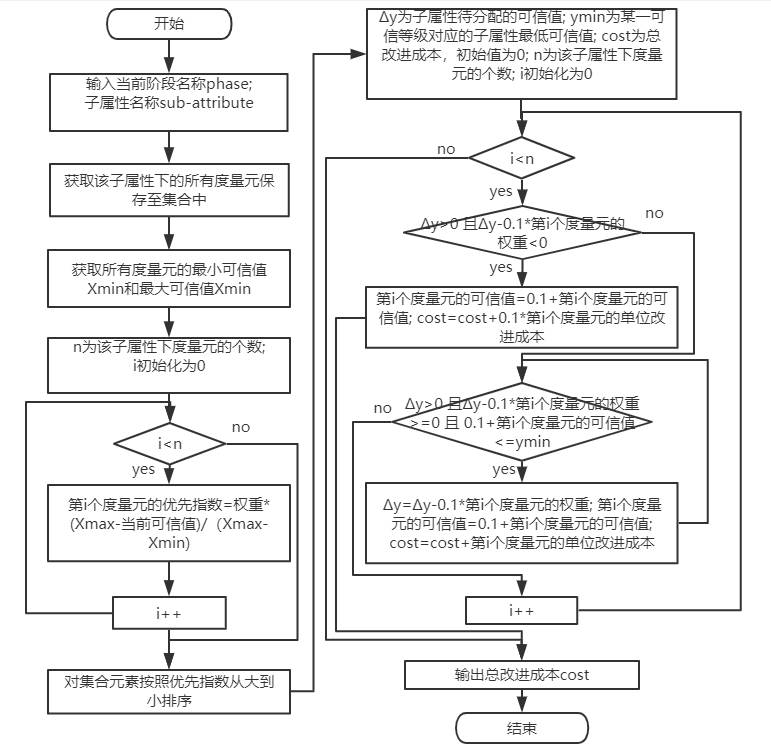
\includegraphics[width=15cm,height=19cm]{fig/4_1.png}
	\caption{算法\uppercase\expandafter{\romannumeral1}流程图}
	\label{fig:4_01}
\end{figure}


\begin{algorithm}
	\caption{基于改进优先指数的可信性分配算法.}
	\label{}
	\begin{algorithmic}[1]
		\REQUIRE current phase, $phase$;
		         current sub-attribute, $subAttribute$;
		\ENSURE total cost, $cost$;
		\STATE get all measure data list $list$ of current sub-attribute;
		\STATE get the max trustworthy value $x_{max}$ and the min trustworthy value $x_{min}$ of metricIndex;
		\STATE $n$ is the length of list;
		\FOR{$i=1$; $i<n$; $i++$}
		 \STATE m->priority=m->weight * $\frac{x_{max}-m->tValue}{x_{max}-x_{min}}$
		\ENDFOR
		\STATE Collections->sort(list)
		\FOR{$i=1$; $i<n$; $i++$}
		 \IF{$\Delta y>0$ and $\Delta y-0.1*m->weight<0$}
		  \STATE m->tValue=0.1+m->tValue
		  \STATE cost=cost+0.1*m->cost
		  \STATE break
		 \ENDIF
		 \WHILE{$\Delta y>0$ and $\Delta y-0.1*m->weight>=0$ and $0.1+m->tValue<=y_{min}$}
		  \STATE $\Delta y=\Delta y-0.1*m->weight$
		  \STATE m->tValue=0.1+m->tValue
		  \STATE cost=cost+0.1*m->cost
		 \ENDWHILE
		\ENDFOR
		\RETURN $cost$
		\STATE end function
	\end{algorithmic}
\end{algorithm}
  
如果有N个度量元,算法的时间复杂度为O(n),空间复杂度为O(n)。


\subsection{可信性分配示例\uppercase\expandafter{\romannumeral1}}
以需求阶段的安全完善性这个子属性为例,当前软件的可信等级为$\uppercase\expandafter{\romannumeral3}$级,安全完善性的可信值为7.82。现在要将软件的可信等级提高到$\uppercase\expandafter{\romannumeral4}$级,根据可信量化分级模型表,子属性可信值最低要达到8.5,则待提升可信值为0.68。假设度量元的单位改进成本为表格中数值。接下来将按照算法的流程,将子属性可信值分配给度量元,并计算提高到$\uppercase\expandafter{\romannumeral4}$级需要投入的成本。
\begin{table}[!ht]
	\centering
	\renewcommand\arraystretch{1.3}
	\caption{可信性分配示例}
	\begin{tabular}{|c|c|c|c|c|}
		\hline
		\textbf{度量元名称} & \textbf{权重} & \textbf{可信值} & \textbf{优先指数} & \textbf{单位改进成本} \\ 
		\hline
		通用安全需求 & 0.14 & 8 & 0.04 & 2  \\
		\hline
		特定安全需求 & 0.05 & 3 & 0.05 & 6 \\
		\hline
		软件安全性工作定义完整 & 0.49 & 7 & 0.21 & 4\\
		\hline
		安全功能需求  &  0.24 & 10 & 0  &8 \\
		\hline
		安全性需求标识 & 0.08 & 10 & 0 & 5 \\
		\hline
	\end{tabular}
	\label{tab-4-5}
\end{table}

首先计算度量元的优先指数分别为[0.04,0.05,0.21,0,0]。按照优先级高先分配的原则,先将可信值分配给优先指数大的度量元。第三个度量元的优先指数最大,度量元可信值提高1.3个单位之后变成8.3,子属性待分配可信值为0.043,此时研发成本为5.2;接下来分配第二个度量元,度量元可信值提高0.8个单位增加到3.8,子属性待分配可信值剩余0.003,研发成本为10;子属性剩余可信值分配给下一个度量元,不足以让度量元的可信值提升0.1个单位,此时,按照0.1单位计算,可信值提高到8.1。总改进成本为10.2。

\subsection{可信性分配算法\uppercase\expandafter{\romannumeral2}}
在实际的项目中,某些度量元的优先指数高,但改进成本可能小于优先指数低的度量元的成本。在基于优先指数的可信性分配算法中,是按照度量元的优先指数从大到小进行分配。本节中,称度量元使子属性提高1单位可信值需要花费的成本为单位贡献成本。比如,安全完善性这个子属性下特定安全需求度量元的单位改进成本为6,权重为0.05,则该度量元的单位贡献成本为$6*\frac{1}{0.05}=120$,意义是如果安全完善性这个子属性下其他度量元保持不变,只通过改变特定安全需求这个度量元使安全完善性的可信值提高1个单位,需要消耗的成本为120。每个度量元的单位贡献成本越低,总成本越低,局部最优满足全局最优,可使用贪心法解决。具体方法:将度量元的单位贡献成本按照从小到大的顺序排列,先选择单位贡献成本小的,循环下去,直至不能再选,所得到的成本为改进子属性可信值需要的最低成本。度量元可信值每次仍然以0.1单位进行迭代增加。图\ref{fig:4_02}为算法流程图。
\begin{figure}[H]
	\centering
	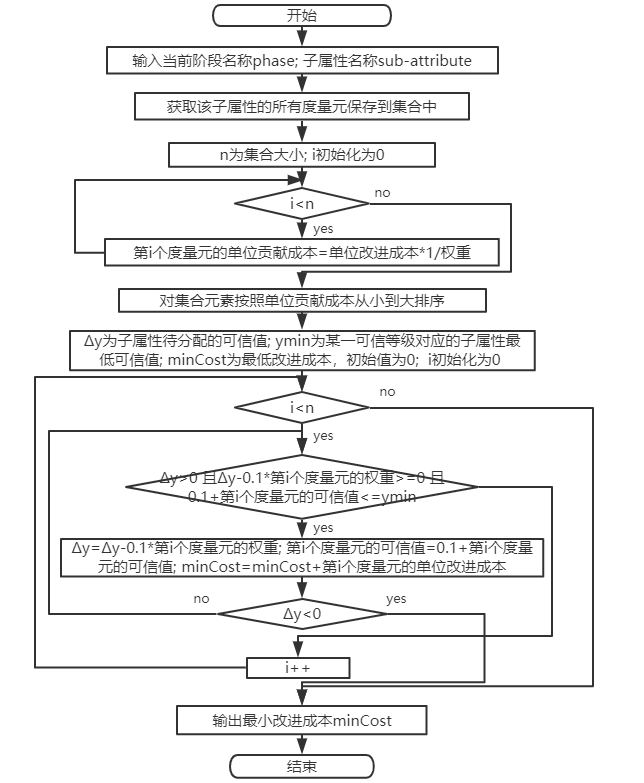
\includegraphics[width=13cm]{fig/4_2.png}
	\caption{算法\uppercase\expandafter{\romannumeral2}流程图}
	\label{fig:4_02}
\end{figure}
\begin{algorithm}
	\caption{基于单位贡献成本可信性分配算法.}
	\label{}
	\begin{algorithmic}[1]
		\REQUIRE current phase, $phase$;
		         current sub-attribute, $subAttribute$;
		\ENSURE total cost, $minCost$;
		\STATE get all measure data list $list$ of current sub-attribute;
		\STATE $n$ is the length of list;
		\FOR{$i=1$; $i<n$; $i++$}
		 \STATE m->conCost=m->cost * $\frac{1}{m->weight}$
		\ENDFOR
		\STATE Collections->sort(list){sort by the conCost value from small to large}
		\FOR{$i=1$; $i<n$; $i++$}
		 \WHILE{$\Delta y>0$ and $0.1+m->tValue<=y_{min}$}
		  \STATE $\Delta y=\Delta y-0.1*m->weight$
		  \STATE m->tValue=0.1+m->tValue
		  \STATE minCost=minCost+0.1*m->cost
		  \IF{$\Delta <0$}
		   \STATE break
		  \ENDIF
		 \ENDWHILE
		\ENDFOR
		\RETURN $minCost$
		\STATE end function
	\end{algorithmic}
\end{algorithm}


假设度量元的个数为N,获得子属性的所有度量元的时间复杂度为O(n),求每个度量元的单位贡献成本时间复杂度为O(n),对每个度量元按照单位贡献成本从小到大排序时间复杂度为O(nlgn),接下来的双重循环时间复杂度为O(n)*常数,所以算法的时间复杂度为O(nlgn),空间复杂度为O(n)。


\subsection{可信性分配示例\uppercase\expandafter{\romannumeral2}}
表\ref{tab-4-6}是考虑度量元单位改进成本的可信值分配示例。
\begin{table}[!ht]
	\centering
	\renewcommand\arraystretch{1.3}
	\caption{基于单位贡献成本的可信性分配示例}
	\begin{tabular}{|c|c|c|c|c|c|}
		\hline
		\textbf{度量元名称} & \textbf{权重} & \textbf{可信值} & \textbf{单位改进成本} & \textbf{单位贡献成本}\\ 
		\hline
		通用安全需求 & 0.14 & 8 & 2 & 14.29 \\
		\hline
		特定安全需求 & 0.05 & 3 & 6 & 120\\
		\hline
		\tabincell{c}{软件安全性工作\\定义完整} & 0.49 & 7 & 4 & 8.16\\
		\hline
		安全功能需求  &  0.24 & 10 & 8 &  33.33  \\
		\hline
		安全性需求标识 & 0.08 & 10  & 5 &  62.5  \\
		\hline
	\end{tabular}
	\label{tab-4-6}
\end{table}

软件当前的可信等级为$\uppercase\expandafter{\romannumeral3}$级,为使软件可信等级达到$\uppercase\expandafter{\romannumeral4}$级,子属性可信值需要提高0.68个单位。按照度量元的单位贡献成本从小到大进行分配,其中第三个度量元单位贡献成本最低,其可信值每次增加0.1,增加了14次之后,可信值变为8.4,子属性可信值已经被分配完毕,此时改进的最低成本为$14*0.1*4=5.6$。







